\documentclass{article}
\usepackage{amsmath}
\usepackage{braket}
\usepackage{MnSymbol}
\usepackage{hyperref}
\usepackage{graphicx}
\usepackage{tikz}
\begin{document}
\textbf{\Large 3.3 Matrices}
\\
\\
We mentioned that operators can be represented as matrices when the vetors are represented as row or column vetors.
Therefore, it is important to understand some of the important properties of matrices.
\\
\\
\\
\textbf{\textit{\large 3.3.1 Eigenvalues and Eigenvectors}}
\\
\\
A matrix maps (transforms) a vector to another vector. For a given matrix, there is a set of vectors
to which it only scales by a scalar when it is applied. These vectors are called the \textbf{eigenvectors} of the matrix.
The corresponding amounts it scales are the \textbf{eigenvalues} of the matrix. For example, if $\ket{i}$ is an eigenvector of \textit{\textbf{M}}, then

\begin{equation} \label{3.7}
    \textit{\textbf{M}} \ket{i}=\lambda_{i}\ket{i}, \tag{3.7}
\end{equation}
\\
where $\lambda_{i}$ is a scalar and the eigencalue of \textit{\textbf{M}}, corresponding to the eigenvector, $\ket{i}$.


For an n$\times$n matrix, it has \textit{n} eigenvalues (counting multiplicities) over the complex field (the eigenvalues can be complex or real). For the same operator, it can be represented in a different matrix form if a different basis is chosen. For some
matrices (\textbf{diagonalizable} matrices), if the eigenvectors are chosen to be the basis states (\textbf{digenbasis}), then the matrix is a diagonal matrix with the eigenvalues alond the diagonal,

\begin{align*} \label{eq 3.8}
    \textit{\textbf{M}}=\begin{pmatrix}
        \lambda_{0} & 0 & \cdots & 0\\
       0 & \lambda_{1} & \cdots & 0 \\
       \vdots & \vdots & \ddots & \vdots\\
       0 & 0 & \cdots & \lambda_{n-1}\\
    \end{pmatrix}_{In \ M's \ eigenbasis} \tag{3.8}
\end{align*}


The process of finding the eigen basis so that the matrix is in a diagonal form is called the \textbf{diagonalization}.diagonalization is a very important tool in solving the Schr\"{o}dinger equation. Note again that \textit{not all matrices are diagonalizable}. Readers are euncourgaed to refer to Section 9.2 in [1] to review how to find the eigenvalues and eigenvectors and, thus, the diagonalization of a matrix.

If the eigenvectors and eigenvalues are given, we can also construct the matrix from the eigenvectros and eigenvalues using this equation,

\begin{equation} \label{eq 3.9}
    \textit{\textbf{M}}=\sum_{i=0}^{n-1}\lambda_{i}\ket{i}\bra{i}. \tag{3.9}
\end{equation}


This is trivial if the matrix is in the eigenbasis which has the form of Eq.(3.8). This is still true in general and can be proved by using the basis transfromation to be discussed in Sect. 3.3.5.
\\
\\
\\
\textit{\textbf{\large 3.3.2 Hermitian Matrix}}
\\
\\
We discussed earlier that the adjoint of an operator \textbf{\textit{M}} is written as 
$\textbf{\textit{M}}^{\dagger}$. When it is written as a matrix, the adjoint of \textbf{\textit{M}}
is its conjugate transpose. If the adjoint of a matrix equals itself, it is also called a \textbf{self-adjoint}
or \textbf{Hermitian} matrix. 
\\
\textbf{Example 3.1} Show that $\sigma_{y}=\begin{pmatrix}
    0 & -i\\ i &0
\end{pmatrix}$ is Hermitian.

\begin{align} \label{eq 3.10}
    \begin{split}
        \sigma_{y}^\dagger&=\begin{pmatrix}
            0 & -i\\ i &0 
        \end{pmatrix}^{T*},\\
        &=\begin{pmatrix}
            0 & -i\\ i &0
        \end{pmatrix}^*,\\
        &=\begin{pmatrix}
        0 & -i\\ i &0
        \end{pmatrix}
        = \sigma_{y}.
    \end{split} \tag {3.10}
\end{align} 

Therefore, it is Hermitian. Here $\sigma_{y}^{T*}$ refers to applying
a transpose operation followed by complex conjugation to $\sigma_{y}$.\hfill $\blacksquare$
\\
\\
\\
\textit{\textbf{\large 3.3.3 Projection Operator}}\\
\\
A projection operator, \textit{\textbf{P}}, is an operator that staisfies the following equation.
\begin{equation}
    \textit{\textbf{P}}=\textit{\textbf{P}}\textit{\textbf{P}}, \tag{3.11}
\end{equation}
which means that applying it twice is the same as applying it once (idempotent).
For our purpose, we want to be more specific on what it does. Therefore, we will label it as 
$\textit{\textbf{P}}_{\ket{v}}$ to indicate that it can be an operator to extract the
$\ket{v}$ component from any vectors. $\ket{v}$ needs to be a \textit{normalized} vector
Therefore, $\braket{v|v}=1$ (see Eq. (2.25) and after). For example, $\textit{\textbf{P}}_{\ket{v}}\ket{\alpha}$
should give us the $\ket{v}$ component in $\ket{\alpha}$. To construct
$\textit{\textbf{P}}_{\ket{v}}$, we can use this equation,

\begin{equation} \label{eq 3.12}
    \textit{\textbf{P}}_{\ket{v}}=\ket{v}\bra{v}. \tag{3.12}
\end{equation}


Let us two examples to understand better.
\\ \\ 
\textbf{Example 3.2} Show $\textit{\textbf{P}}_{\ket{v}}=\textit{\textbf{P}}_{\ket{v}}\textit{\textbf{P}}_{\ket{v}}$.

\begin{align} \label{eq 3.13}
    \begin{split}
        \textit{\textbf{P}}_{\ket{v}}\textit{\textbf{P}}_{\ket{v}}&=(\ket{v}\bra{v})(\ket{v}\bra{v}),\\
        &=\ket{v}(\braket{v|v})\bra{v},\\
        &=\ket{v}\bra{v},\\
        &=\textit{\textbf{P}}_{\ket{v}}
    \end{split} \tag{3.13}
\end{align}

Therefore, as long as $\ket{v}$ is \textit{normalized} vector,$\textit{\textbf{P}}_{\ket{v}}$
satisfies the definition of a projection operator.\hfill $\blacksquare$
\\\\
\textbf{Example 3.3} In a 1-qubit system, a general state can be written as $\ket{\psi}=\alpha\ket{0}+\beta\ket{1}$.
Find the $\ket{0}$ component of $\ket{\psi}$ is $\alpha\ket{0}$ from the given expresson.
Let us use the projection operator to find it, too. Firstly, we recall that the column and row representation of $\ket{0}$ and $\bra{0}$
are, 

\begin{align} \label{eq 3.14}
    \begin{split}
        \ket{0} &= \begin{pmatrix}
            1 \\ 0
        \end{pmatrix},\\
        \bra{0} &= \begin{pmatrix}
            1 \ 0\\
        \end{pmatrix}.
    \end{split} \tag{3.14}
\end{align}

Therefore, the projection operator for $\ket{0}$ is

\begin{align} \label{eq 3.15}
    \begin{split}
        \textit{\textbf{P}}_{\ket{0}}&= \ket{0}\bra{0},\\
        &=\begin{pmatrix}
            1 \\0
        \end{pmatrix}
        \begin{pmatrix}
            1 \ 0
        \end{pmatrix},\\
        &= \begin{pmatrix}
            1 \ 0\\ 0 \ 0
        \end{pmatrix}.
    \end{split} \tag{3.15}
\end{align}\\
We may use two methods to find the answer. Firstly, by using \textit{bra-ket} notation, we have,

\begin{align} \label{eq 3.16}
    \begin{split}
        \textbf{\textit{P}}_{\ket{0}} \ket{\psi} &=\begin{pmatrix}
            1 \ 0 \\ 0 \ 0
        \end{pmatrix}
        \begin{pmatrix}
            \alpha \\ \beta
        \end{pmatrix},\\
        &=\begin{pmatrix}
            \alpha \\ 0
        \end{pmatrix},\\
        &= \alpha \begin{pmatrix}
            1 \\ 0
        \end{pmatrix} = \alpha \ket{0}.
    \end{split} \tag{3.16}
\end{align}

Both methods gice the same result as expected. \hfill $\blacksquare$
\\\\
\textit{\textbf{\large 3.3.4 Unitary Matrix }}
\\\\
A \textbf{unitary matrix}, \textit{\textbf{U}}, is a matrix that satisfies the following equations:

\begin{align} \label{eq 3.18}
    \begin{split}
        \textit{\textbf{U}}\textit{\textbf{U}}^\dagger&=\textit{\textbf{U}}^\dagger\textit{\textbf{U}}=\textit{\textbf{I}}, \\
       \textit{\textbf{U}}^\dagger &= \textit{\textbf{U}}^{-1}.
    \end{split} \tag{3.18}
\end{align}

Unlike a HErmitian matrix which is equal to its adjoint, a unitary matrix has its \textbf{inverse} equal to
its adjoint. The most important property of a unitary matrix is that it preserves
the inner product of two vetors when both vectors are transformed by 
the same unitary matrix. For eample, after the transformation, vectors $\ket{g}$ and $\ket{f}$
become $\ket{g^\prime}=\textit{\textbf{U}}\ket{g}$ and $\ket{f^\prime}=\textit{\textbf{U}}\ket{f}$,
respectively. The inner producto of the new vectors is

\begin{align} \label{eq 3.19}
    \begin{split}
        \braket{g^\prime|f^\prime}&=(\bra{g}\textit{\textbf{U}}^{\dagger})(\textit{\textbf{U}}\ket{f}),\\
    &=\bra{g}(\textit{\textbf{U}}^{\dagger}\textit{\textbf{U}})\ket{f},\\
        &= \braket{g|\;\textit{\textbf{I}} \;|f},\\
        &=\braket{g|f},
\end{split} \tag{3.19}
\end{align}

where Eqs. (3.4) and (\ref{eq 3.18}) are used in line 1 and line 3, respectively. Since a unitary matrix presreces the inner product of two vectors, it also 
\textit{preserves the norm} of any vectors as the norm of a vector is just the quare root of the inner product of the vector to itself (Eq. (2.7)).
Therefore, later we will see that a quantum gate must be unitary so that the state vector norm is not changed after each operation and keeps normalized.


It should also he noted that when a unitary matrix is written in matrix form, each
of its colums is a normalized vector and is orthogonal to other columns. This is
the same for the rows. this means that if the matrix is,

\begin{align} \label{eq 3.20}
    \begin{split}
        \textit{\textbf{U}}&=\begin{pmatrix}
            b_{0,0} & b_{0.1} & \cdots & b_{0,n-1}\\
            b_{1,0} & b_{1.1} & \cdots & b_{1,n-1}\\
            \vdots & \vdots & \ddots & \vdots\\
            b_{n-1,0} & b_{n-1.1} & \cdots & b_{n-1,n-1}\\
        \end{pmatrix},\\
        &=(\ket{v_0}\ket{v_1}\cdots\ket{v_{n-1}}),
    \end{split} \tag{3.20}
\end{align}

where we have set
\begin{equation} \label{eq 3.21}
    \ket{v_i}=\begin{pmatrix}
        b_{o,i}\\
        b_{1,i}\\
        \vdots\\
        b_{n-1,i}\\
    \end{pmatrix}, \tag{3.21}
\end{equation} 

then we have 

\begin{equation} \label{eq 3.22}
    \braket{v_i|v_j}=\delta_{i,j}, \tag{3.22}
\end{equation}\\ \\
\textit{\textbf{\large 3.3.5 Transformation of Basis}}
\\\\
Sometimes we want to work on a different basis for convenience. Then 
we need to perform an appropriate transformation of the vectors and matrices.
For exampe, in Fig 3.1, vector $\ket{V}$ might be originally represented in the old
basis $\ket{0}/\ket{1}$ as $\ket{V}=\alpha_0\ket{0}+\alpha_1\ket{1}$.
We want to find its representation in a new basis $\ket{0^\prime}/\ket{1^\prime}$
and it might be $\ket{V}=\alpha^\prime_0\ket{0^\prime}+\alpha^\prime_1\ket{1^\prime}$.
We have done somtheing similar in Fig. 2.2. Here we want to show an equation to help us
perform the transformation.

Suppose an \textit{n}-dimensional vector is represented in a vector form with the basis vectors in the old
basis being $\ket{0},\ket{1},\cdots,\ket{n-1}$. Now we want to represent it in
a new basis with basis vectors $\ket{0^\prime},\ket{1^\prime},\cdots,\ket{n-1^\prime}$.
The transformation matrix
\\\\


\begin{center}

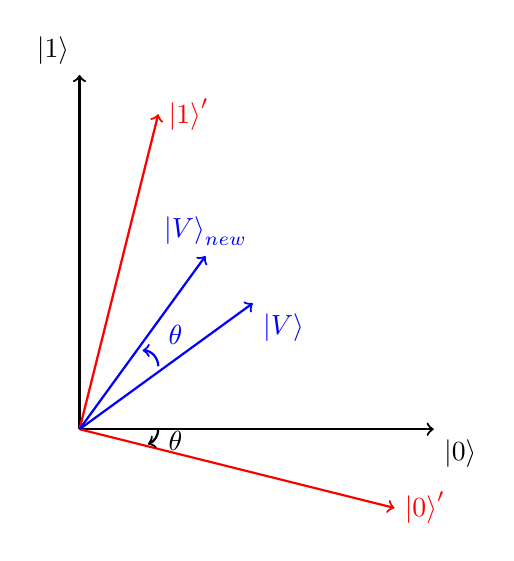
\begin{tikzpicture}
    \draw[thick,->] (0,0)--(4.5,0) node[anchor=north west] {$\ket{0}$};
    \draw[thick,->] (0,0)--(0,4.5) node[anchor=south east] {$\ket{1}$};
    \draw[thick,->,color=red] (0,0)--(1,4) node[anchor=west] {$\ket{1}^\prime$};
    \draw[thick,->,color=red] (0,0)--(4,-1) node[anchor=west] {$\ket{0}^\prime$};
    \draw[thick,->,color=blue] (0,0)--(1.6,2.2) node [anchor=south] {$\ket{V}_{new}$};
    \draw[thick,->,color=blue] (0,0)--(2.2,1.6) node[anchor=north west]{$\ket{V}$};
    \draw[thick,->,color=blue] (1,0.8) arc (0:90:0.2cm) node[anchor=west] at (1,1.2) {$\theta$};
    \draw[thick,->] (1,0) arc (0:-70:0.2cm) node[anchor=west] at (1,-0.15) {$\theta$};
\end{tikzpicture}
    
\end{center}
Fig.3.1 Representation of vector $\ket{V}$ in the new basis $\ket{0^\prime}/\ket{1^\prime}$ 
is the same as the representatino of vector $\ket{V}_{new}$ in the old basis $\ket{0}/\ket{1}$
\\
to represnet a vector in the new basis is given by

\begin{equation} \label{eq 3.23}
    \textit{\textbf{U}}=\begin{pmatrix}
        \braket{0^\prime|0}&\braket{0^\prime|1}&\cdots&\braket{0^\prime|n-1}\\
        \braket{1^\prime|0}&\braket{1^\prime|1}&\cdots&\braket{1^\prime|n-1}\\
        \vdots&\vdots&\ddots&\vdots\\
        \braket{n-1^\prime|0}&\braket{n-1^\prime|1}&\cdots&\braket{n-1^\prime|n-1}\\        
    \end{pmatrix}. \tag{3.23}
\end{equation}

By using this matrix, we can fidn the coefficients of the vector in the new basis
through matrix multiplication.

\begin{equation} \label{eq 3.24}
    \begin{pmatrix}
        \alpha^\prime_0\\
        \alpha^\prime_1\\
        \vdots\\
        \alpha^\prime_{n-1}\\
    \end{pmatrix}=
    \begin{pmatrix}
        \braket{0^\prime|0}&\braket{0^\prime|1}&\cdots&\braket{0^\prime|n-1}\\
        \braket{1^\prime|0}&\braket{1^\prime|1}&\cdots&\braket{1^\prime|n-1}\\
        \vdots&\vdots&\ddots&\vdots\\
        \braket{n-1^\prime|0}&\braket{n-1^\prime|1}&\cdots&\braket{n-1^\prime|n-1}\\        
    \end{pmatrix}
    \begin{pmatrix}
         \alpha_0\\
        \alpha_1\\
        \vdots\\
        \alpha_{n-1}\\
    \end{pmatrix}. \tag{3.24}
\end{equation}

We may better apprecieate the meaing of this equation if we realize that the \textit{i}-th
row of the left-hand side ($\alpha_{i}^\prime$), which represents the amount of $\ket{i^\prime}$
component in the new basis, is the sum of the amount of each componenet
in the old basis (e.g., $\alpha_j$) weighted by their ovelats (commons) with $\ket{i^\prime}$, i.e., $\braket{i^\prime|j}$.

Equation (\ref{eq 3.24}) also reveals another important thing. As discussed,
a matrix applying to a vector is also a transformation of the vector. Therefore, the left-hand
side can also be regarded as a new vector $\ket{V}_{new}$ after a certain operation \textit{in the old basis}.
What is this opration? As shown in Fig. 3.1, if the new basis can be obtained
by rotating the old basis clockwsie by an angle, $\theta$, the operation is equibalent to a
counterclockwise rotation fo the vector by an angle, $\theta$, in the old basis.
In the figure, it can be seen that the representation of vector $\ket{V}$ in the new
basis $\ket{0^\prime}/\ket{1^\prime}$ is the same as the representation of vector
$\ket{V}_{new}$ in the old basis $\ket{0}/\ket{1}$. In general, when we represent a vector in a new basis 
formed by a transformation $\textit{\textbf{U}}^{-1}$ of the old basis, it is the same as 
transforming the vector in the old basis by its inverse, i.e., \textit{\textbf{U}}.
\\\\
\textbf{Example 3.4} For the problem in Gif.2 2.2, construct the transformation matrix to 
convert the representation of $\ket{V_1}$ in the old $\ket{0}\ket{1}$
basis to the new $\ket{+}/\ket{-}$ basis.

Firstly, we recognize that the old basis has basis vector $\ket{0}$
and $\ket{1}$. The new basis has basis vectors $\ket{0^\prime}=\ket{+}$ and
$\ket{1^\prime}=\ket{-}$. Therefore, the transformation matrix is 
\begin{align} \label{eq 3.25}
    \begin{split}
        \textit{\textbf{U}} &= \begin{pmatrix}
            \braket{0^\prime|0} \ \braket{0^\prime|1}\\
            \braket{1^\prime|0} \ \braket{1^\prime|1}\\
        \end{pmatrix}
        =\begin{pmatrix}
        \braket{+|0} \ \braket{+|1}\\
            \braket{-|0} \ \braket{+|1}\\    
        \end{pmatrix},\\
        &=\begin{pmatrix}
            \frac{1}{\sqrt{2}} & \frac{1}{\sqrt{2}}\\
            \frac{1}{\sqrt{2}} & -\frac{1}{\sqrt{2}}\\
        \end{pmatrix}
        =\frac{1}{\sqrt{2}}\begin{pmatrix}
            1 &1 \\ 1 & -1\\
        \end{pmatrix}. 
    \end{split}\tag{3.25}
\end{align}
Now, if we apply \textit{\textbf{U}} to $\ket{V_1}=\ket{0}$ as given
in the first line of Eq.(2.15), we gate

\begin{equation} \label{eq 3.26}
    \textit{\textbf{U}}\ket{V_1}=\frac{1}{\sqrt{2}}\begin{pmatrix}
        1&1\\1&-1\\
    \end{pmatrix}
    \begin{pmatrix}
        1\\0
    \end{pmatrix}
    =\frac{1}{\sqrt{2}}\begin{pmatrix}
        1\\1
    \end{pmatrix}. \tag{3.26}
\end{equation}
which has the same coefficients as those in the last line of Eq. (2.15).
As discussed, $\textit{\textbf{U}}\ket{V_1}$ is also the vector formed after rotating 
$\ket{V_1}$ counterclockwise by 45$^o$ in the old basis.\hfill $\blacksquare$

If two vectors $\ket{g}$ and $\ket{f}$ are represented in a new basis, we expect that their inner product will not change. 
Since representing the vectors in a new basis is equibalent to tranforming the vetors in the old basis,
i.e., $\ket{g^\prime}=\textit{\textbf{U}}\ket{g}$ and $\ket{f^\prime}=\textit{\textbf{U}}\ket{f}$,
then it means that \textit{the transformation matrix must be unitary} in order to
preserve their inner product (See Eq. {\ref{eq 3.19}}). Therefore, it also obets Eq ({\ref{eq 3.18}}),
i.e., $\textit{\textbf{U}}^\dagger\textit{\textbf{U}}=\textit{\textbf{I}}$.

Similar to vectors, when the basis is changed, matrices also need to be transformed accordingly.
A matrix \textit{\textbf{M}} is transformed to $\textit{\textbf{M}}^\prime$ through

\begin{equation} \label{eq 3.27}
    \textit{\textbf{M}}^\prime= \textit{\textbf{U}}\textit{\textbf{M}}\textit{\textbf{U}}^\dagger.\tag{3.27}
\end{equation} 


This is also called the \textbf{similarity transformation}. It is not diffcult to see that this makes sense. Assume
$\ket{w}=\textit{\textbf{M}}\ket{v}$. This means that vector $\ket{v}$ is transformed
by an operator \textit{\textbf{M}} to another vector $\ket{w}$ and they are all in the same
old basis. Now if we want to work on a new basis by applying the basis transformation matrix 
\textit{\textbf{U}}, we have,

\begin{align} \label{eq 3.28}
    \begin{split}
        \textit{\textbf{U}} \ket{w} &= \textit{\textbf{U}}(\textit{\textbf{M}} \ \ket{v}),\\
        &= \textit{\textbf{U}} \ \textit{\textbf{M}} \ \textit{\textbf{I}}\ket{v},\\
        &= \textit{\textbf{U}} \ \textit{\textbf{M}} \ (\textit{\textbf{U}}^\dagger\textit{\textbf{U}})\ket{v},\\
        &= (\textit{\textbf{U}} \ \textit{\textbf{M}} \ \textit{\textbf{U}}^\dagger)\textit{\textbf{U}}\ket{v},\\
    \end{split} \tag{3.28}
\end{align}

which clearly shows that $\ket{w}$ in the new basis (\textit{\textbf{U}}$\ket{w}$) equals the operator in the new
basis ($(\textit{\textbf{U}} \ \textit{\textbf{M}} \ \textit{\textbf{U}}^\dagger$), Eq. (\ref{eq 3.27})) multiplying $\ket{v}$ in the new basis
 ($\textit{\textbf{U}}\ket{v}$). 
 This preserves the relationship between the vectors in the old basis, i.e., $\ket{w}=\textit{\textbf{M}}\ket{v}$. 
 
\end{document}